\chapter{Alegeri legate de Hiperparametri și Antrenare}
\label{sec:architecture}

Două decizii principale se aplică uniform pentru toate modelele și seturile de date:

\begin{itemize}
  \item \textbf{Optimizator.} Toate rețelele neuronale sunt antrenate cu Adam, la o rată de învățare fixă de $10^{-3}$, uniform pentru fiecare model și set de date.
  \item \textbf{Fără căutare de hiperparametri.} Dacă un model a avut performanțe neașteptat de slabe, rata sa de învățare a fost verificată suplimentar cu $\{10^{-4}, 10^{-3}, 3\times10^{-3}\}$ înainte de a trage vreo concluzie din acel rezultat.
  \item \textbf{Partiție de validare doar pentru monitorizare.} Fiecare rețea neuronală reține aleator 10\% din datele de antrenare exclusiv pentru a trasa o curbă de pierdere (\emph{loss}) de antrenare/validare per rulare, ca verificare că antrenarea decurge corect. Această partiție nu este niciodată folosită pentru oprire timpurie (\emph{early stopping}) sau selecția modelului: antrenarea rulează întotdeauna pentru numărul fix de epoci de mai jos, iar rezultatele raportate pe setul de testare folosesc ponderile modelului din epoca finală.
\end{itemize}

\section{Isolation Forest}

\begin{center}
\begin{tabular}{@{}lllll@{}}
\toprule
 & CIC flat & CIC context & Yahoo & Credit card \\
\midrule
N\_ESTIMATORS & 150 & 150 & 150 & 150 \\
MAX\_SAMPLES & 300{,}000 & 300{,}000 & $\min(n, 50{,}000)$ & 200{,}000 \\
Dimensiunea setului de antrenare & $\sim$371k & $\sim$371k & câteva mii & $\sim$227k \\
\% din antrenare folosit & $\sim$81\% & $\sim$81\% & $\sim$100\% & $\sim$88\% \\
RANDOM\_SEED & 123 & 123 & 123 & 123 \\
\bottomrule
\end{tabular}
\end{center}

\texttt{MAX\_SAMPLES} este singura diferență semnificativă și este setat cât mai ridicat posibil, practic, pentru fiecare set de date (acuratețea crește odată cu mai multe eșantioane per arbore, cu randamente descrescânde;
problema de \enquote{swamping} al arborilor nu apare aici, întrucât datele de antrenare sunt întotdeauna exclusiv benigne). Plafonul de 50.000 pentru Yahoo nu este atins niciodată în practică și este păstrat doar ca limită de siguranță.

\section{One-Class SVM}

\begin{center}
\begin{tabular}{@{}lllll@{}}
\toprule
 & CIC flat & CIC context & Yahoo & Credit card \\
\midrule
NU & 0.01 & 0.01 & 0.01 & 0.01 \\
KERNEL & rbf & rbf & rbf & rbf \\
GAMMA & scale & scale & scale & scale \\
SUBSAMPLE & 50{,}000 & 50{,}000 & niciunul (complet) & niciunul (complet) \\
\% din antrenare folosit & $\sim$13.5\% & $\sim$13.5\% & $\sim$100\% & $\sim$100\% \\
\bottomrule
\end{tabular}
\end{center}

Toți parametrii kernel/nu sunt uniformi pe seturile de date. Subeșantionarea este aplicată doar acolo unde setul de antrenare este suficient de mare încât un OC-SVM pe toate datele ar deveni mult prea lent; credit card ($\sim$227k rânduri) a fost antrenat pe tot setul, fără subeșantionare.

\section{Autoencoder Feedforward (MLP)}

\begin{center}
\begin{tabular}{@{}lllll@{}}
\toprule
 & CIC flat & CIC context & Yahoo & Credit card \\
\midrule
Dimensiune intrare & 77 & 86 & 64 (fereastră aplatizată) & $\sim$30 (PCA) \\
Dimensiuni ascunse & [64, 32, 16] & [64, 32, 16] & [32, 16] & [16, 8] \\
Raport bottleneck & 0.21 & 0.19 & 0.25 & $\sim$0.27 \\
Activare finală & Sigmoid & Sigmoid & Linear & Linear \\
\bottomrule
\end{tabular}
\end{center}

Lățimile straturilor sunt scalate în funcție de dimensiunea intrării, astfel încât raportul de compresie al bottleneck-ului să rămână aproximativ constant ($\sim$0.20--0.27) pe toate seturile de date. Activarea finală diferă întrucât CIC folosește \texttt{MinMaxScaler} (mărginit la $[0,1]$, potrivit pentru o ieșire sigmoid), în timp ce Yahoo și credit card folosesc scalere nemărginite (ieșire liniară).

\section{LSTM Predictiv}

\begin{center}
\begin{tabular}{@{}llll@{}}
\toprule
 & CIC & Yahoo & Credit card \\
\midrule
INPUT\_SIZE & 77 & 1 & 1 \\
HIDDEN\_DIM & 128 & 64 & 64 \\
NUM\_LAYERS & 1 & 1 & 1 \\
EPOCHS & 20 & 20 & 50 \\
BATCH\_SIZE & 256 & 256 & 512 \\
\bottomrule
\end{tabular}
\end{center}

\texttt{HIDDEN\_DIM} este scalat în funcție de dimensiunea intrării pentru CIC (o extindere de $\sim$1.66$\times$ față de cele 77 de caracteristici de intrare); ambele seturi de date univariate folosesc 64, o capacitate suficientă pentru un semnal scalar. Credit card folosește mai multe epoci (50) întrucât curba sa de pierdere continuă să scadă și după epoca 30 -- probabil o consecință directă a tratării celor 29 de caracteristici PCA netemporale ca pseudo-secvență, ceea ce face optimizarea mai zgomotoasă decât pe date cu adevărat temporale. CIC și Yahoo converg până la epoca $\sim$5, deci 20 de epoci este deja o alegere conservatoare pentru acestea.

\section{Autoencoder LSTM}

\begin{center}
\begin{tabular}{llll}
\toprule
 & CIC & Yahoo & Credit card \\
\midrule
INPUT\_SIZE & 77 & 1 & 1 \\
HIDDEN\_DIM & 128 & 64 & 64 \\
NUM\_LAYERS & 1 & 1 & 1 \\
EPOCHS & 50 & 30 & 50 \\
BATCH\_SIZE & 256 & 256 & 512 \\
\bottomrule
\end{tabular}
\end{center}

Atât CIC, cât și credit card au necesitat 50 de epoci pentru a atinge un platou; Yahoo converge până la epoca $\sim$5, deci 30 este deja generos.

\section{Bottleneck Transformer Autoencoder}

\begin{center}
\begin{tabular}{llll}
\toprule
 & CIC & Yahoo & Credit card \\
\midrule
D\_MODEL & 64 & 64 & 64 \\
NHEAD & 4 & 4 & 4 \\
NUM\_LAYERS & 2 & 2 & 2 \\
DIM\_FF & 256 & 256 & 256 \\
LATENT\_DIM & 32 & 32 & 32 \\
EPOCHS & 50 & 20 & 20 \\
BATCH\_SIZE & 256 & 256 & 512 \\
\bottomrule
\end{tabular}
\end{center}

\texttt{LATENT\_DIM=32} oferă o compresie uniformă de 50\% față de \texttt{D\_MODEL=64}, pe toate cele trei seturi de date.

\section{Causal Transformer}

\begin{center}
\begin{tabular}{lll}
\toprule
 & CIC & Yahoo \\
\midrule
D\_MODEL & 64 & 64 \\
NHEAD & 4 & 4 \\
NUM\_LAYERS & 2 & 2 \\
DIM\_FF & 256 & 256 \\
DROPOUT & 0.1 & 0.1 \\
EPOCHS & 30 & 30 \\
BATCH\_SIZE & 256 & 256 \\
\bottomrule
\end{tabular}
\end{center}



\chapter{Protocolul de Evaluare: Metrici și Rezultate Complete}
\label{sec:eval-metrics}

\section{Metrici Raportate}

Fiecare rulare produce un raport text care conține toate metricile din Tabelul~\ref{tab:eval-metrics-def}. Capitolul de Rezultate raportează doar un subset dintre acestea (de obicei ROC-AUC, Precizia Medie, și, unde este relevant, Acuratețea Echilibrată și F1), ales pentru a nu aglomera tabelele de comparație; setul complet, per model și per set de date, este prezentat în \S\ref{sec:eval-full-cc}--\S\ref{sec:eval-full-cic}.

\begin{table}[H]
\centering
\begin{tabular}{@{}p{4cm}p{9.5cm}@{}}
\toprule
Metrică & Note \\
\midrule
Precizie / Recall / F1 (per clasă) & Prin \texttt{sklearn.classification\_report}, raportate atât pentru clasa normală, cât și pentru clasa anomalie, plus acuratețea și mediile macro/ponderate. \\
ROC-AUC & Raportat pentru completitudine / comparabilitate cu literatura anterioară; nu este metrica principală de clasificare în condiții de dezechilibru de clase. \\
Precizie Medie (PR-AUC) & Independentă de prag; alegerea standard în condiții de dezechilibru sever de clase, întrucât ROC-AUC poate părea înșelător de bun atunci când exemplele negative depășesc masiv numărul celor pozitive. \\
Acuratețe Echilibrată & $\frac{1}{2}(\text{sensibilitate} + \text{specificitate})$ la pragul de operare selectat. \\
F1 (clasa pozitivă/atac) & La pragul de operare selectat. \\
Numărători din matricea de confuzie & TP/TN/FP/FN brute, la pragul selectat. \\
\bottomrule
\end{tabular}
\caption{Metrici raportate de fiecare rulare de evaluare.}
\label{tab:eval-metrics-def}
\end{table}

\paragraph{Notă privind consistența numerelor.} Tabelele~\ref{tab:eval-full-cc}--\ref{tab:eval-full-cic} de mai jos completează Capitolul~\ref{ch:results} cu detaliul complet (precizie/recall pe clasa pozitivă, matrice de confuzie) pentru fiecare model. 
Coloanele ROC-AUC / Precizie Medie / Acuratețe Echilibrată / F1 reproduc exact valorile deja publicate în Capitolul~\ref{ch:results}, pentru consistență. Pentru un număr de modele -- în special pe CIC-IDS2017, unde reevaluări ulterioare au schimbat scorurile -- nu toate metricile au mai fost calculate. În aceste cazuri, rândul din tabel afișează doar metricile agregate deja publicate.

\section{Rezultate Complete -- Credit Card Fraud Detection}
\label{sec:eval-full-cc}

\begin{table}[H]
\centering
\resizebox{\textwidth}{!}{%
\begin{tabular}{@{}lcccccccccc@{}}
\toprule
Model & Precizie (fraudă) & Recall (fraudă) & F1 (fraudă) & ROC-AUC & Precizie Medie & Acuratețe Echilibrată & TP & TN & FP & FN \\
\midrule
MLP Autoencoder           & 0.6205 & 0.8008 & 0.6992 & 0.9649 & 0.7105 & 0.8983 & 394 & 56622 & 241 & 98 \\
Isolation Forest          & 0.5000 & 0.7724 & 0.6070 & 0.9587 & 0.6725 & 0.8828 & 380 & 56483 & 380 & 112 \\
LSTM Autoencoder          & 0.6904 & 0.7886 & 0.7362 & 0.9476 & 0.6223 & 0.8928 & 388 & 56689 & 174 & 104 \\
OC-SVM                    & 0.5501 & 0.7805 & 0.6454 & 0.9354 & 0.5959 & 0.8875 & 384 & 56549 & 314 & 108 \\
Transformer Bottleneck AE & 0.5073 & 0.7764 & 0.6137 & 0.9583 & 0.5947 & 0.8849 & 382 & 56492 & 371 & 110 \\
Predictive LSTM           & 0.3992 & 0.7642 & 0.5244 & 0.9581 & 0.5190 & 0.8771 & 376 & 56297 & 566 & 116 \\
\bottomrule
\end{tabular}%
}
\caption{Credit Card Fraud Detection -- toate metricile raportate, pentru toate cele șase modele evaluate.}
\label{tab:eval-full-cc}
\end{table}

\section{Rezultate Complete -- Yahoo Webscope S5}
\label{sec:eval-full-yahoo}

\begin{table}[H]
\centering
\resizebox{\textwidth}{!}{%
\begin{tabular}{@{}lcccccccccc@{}}
\toprule
Model & Precizie (poz.) & Recall (poz.) & F1 (poz.) & ROC-AUC & Precizie Medie & Acuratețe Echilibrată & TP & TN & FP & FN \\
\midrule
\multicolumn{11}{@{}l}{\textbf{A1 -- anomalii punctuale}} \\
MLP Autoencoder  & -- & -- & -- & 0.792 & 0.611 & -- & -- & -- & -- & -- \\
LSTM Autoencoder & 0.2944 & 0.7904 & 0.4290 & 0.794 & 0.600 & 0.6916 & 852 & 2974 & 2042 & 226 \\
OC-SVM           & 0.5183 & 0.5909 & 0.5522 & 0.776 & 0.595 & 0.7364 & 637 & 4424 & 592 & 441 \\
LSTM Predictiv   & 0.2988 & 0.8016 & 0.4354 & 0.789 & 0.588 & 0.6988 & 3442 & 11912 & 8076 & 852 \\
Isolation Forest & 0.2439 & 0.8646 & 0.3805 & 0.765 & 0.511 & 0.6443 & 932 & 2127 & 2889 & 146 \\
\midrule
\multicolumn{11}{@{}l}{\textbf{A3 -- anomalii contextuale/sezoniere}} \\
LSTM Predictiv             & -- & -- & -- & 0.868 & 0.812 & -- & -- & -- & -- & -- \\
Transformer Bottleneck AE  & -- & -- & -- & 0.762 & 0.663 & -- & -- & -- & -- & -- \\
Causal Transformer         & -- & -- & -- & 0.738 & 0.623 & -- & -- & -- & -- & -- \\
MLP Autoencoder            & 0.4247 & 0.9540 & 0.5878 & 0.765 & 0.507 & 0.6622 & 13785 & 10981 & 18670 & 664 \\
LSTM Autoencoder           & 0.3278 & 1.0000 & 0.4937 & 0.566 & 0.392 & 0.5003 & 14449 & 20 & 29631 & 0 \\
OC-SVM                     & 0.3285 & 0.9996 & 0.4945 & 0.584 & 0.376 & 0.5020 & 14443 & 128 & 29523 & 6 \\
Isolation Forest           & 0.3301 & 0.9960 & 0.4959 & 0.511 & 0.331 & 0.5055 & 14391 & 447 & 29204 & 58 \\
\midrule
\multicolumn{11}{@{}l}{\textbf{A4 -- schimbări de nivel}} \\
LSTM Predictiv             & 0.3975 & 0.7951 & 0.5300 & 0.745 & 0.505 & 0.6864 & 9098 & 18868 & 13789 & 2345 \\
Causal Transformer         & 0.3092 & 0.9098 & 0.4616 & 0.695 & 0.436 & 0.5988 & 10411 & 9401 & 23256 & 1032 \\
MLP Autoencoder            & -- & -- & -- & 0.719 & 0.402 & -- & -- & -- & -- & -- \\
Transformer Bottleneck AE  & 0.2625 & 0.9959 & 0.4155 & 0.655 & 0.404 & 0.5077 & 11396 & 636 & 32021 & 47 \\
Isolation Forest           & 0.2595 & 1.0000 & 0.4121 & 0.498 & 0.268 & 0.5001 & 11443 & 6 & 32651 & 0 \\
OC-SVM                     & 0.2603 & 1.0000 & 0.4131 & 0.519 & 0.265 & 0.5021 & 11443 & 139 & 32518 & 0 \\
LSTM Autoencoder           & 0.2644 & 0.9979 & 0.4181 & 0.502 & 0.252 & 0.5127 & 11419 & 895 & 31762 & 24 \\
\bottomrule
\end{tabular}%
}
\caption{Yahoo Webscope S5 -- toate metricile raportate, pe benchmark (A1, A3, A4), ordonate ca în tabelele din Capitolul~\ref{ch:results}.}
\label{tab:eval-full-yahoo}
\end{table}

\section{Rezultate Complete -- CIC-IDS2017}
\label{sec:eval-full-cic}

Compoziția pe clase de atac a setului de test temporal (analoagă Tabelului~\ref{tab:cic-composition} din Capitolul~\ref{ch:results} pentru setul flat/context) este detaliată separat, în Capitolul~\ref{ch:cic-composition-temporal}.

\begin{table}[H]
\centering
\resizebox{\textwidth}{!}{%
\begin{tabular}{@{}llcccccccccc@{}}
\toprule
Model & Set de caracteristici & Precizie (atac) & Recall (atac) & F1 (atac) & ROC-AUC & Precizie Medie & Acuratețe Echilibrată & TP & TN & FP & FN \\
\midrule
MLP Autoencoder            & Context  & -- & -- & -- & 0.9860 & 0.9487 & 0.9548 & -- & -- & -- & -- \\
OC-SVM                     & Context  & 0.8965 & 0.9509 & 0.9229 & 0.9745 & 0.9396 & 0.9569 & 412650 & 1238310 & 47634 & 21327 \\
Isolation Forest           & Context  & -- & -- & -- & 0.9785 & 0.9328 & 0.9270 & -- & -- & -- & -- \\
LSTM Autoencoder           & Temporal & 0.4752 & 0.9126 & 0.6249 & 0.8976 & 0.7955 & 0.7846 & 398793 & 842158 & 440453 & 38212 \\
MLP Autoencoder            & Flat     & -- & -- & -- & 0.9189 & 0.7921 & 0.8022 & -- & -- & -- & -- \\
Isolation Forest           & Flat     & -- & -- & -- & 0.9049 & 0.7612 & 0.8228 & -- & -- & -- & -- \\
OC-SVM                     & Temporal & 0.4214 & 0.9770 & 0.5888 & 0.8629 & 0.7816 & 0.7600 & 426967 & 696384 & 586227 & 10038 \\
MLP Autoencoder            & Temporal & -- & -- & -- & 0.8831 & 0.7509 & 0.7734 & -- & -- & -- & -- \\
Isolation Forest           & Temporal & 0.3577 & 0.9487 & 0.5195 & 0.8438 & 0.7604 & 0.6841 & 414606 & 538115 & 744496 & 22399 \\
OC-SVM                     & Flat     & 0.3045 & 0.9778 & 0.4644 & 0.7336 & 0.6845 & 0.6121 & 424338 & 316815 & 969129 & 9639 \\
Bottleneck Transformer AE  & Temporal & -- & -- & -- & 0.8077 & 0.6539 & 0.7059 & -- & -- & -- & -- \\
Causal Transformer         & Temporal & -- & -- & -- & 0.7099 & 0.5449 & 0.5520 & -- & -- & -- & -- \\
Predictive LSTM            & Temporal & -- & -- & -- & 0.6126 & 0.4472 & 0.5475 & -- & -- & -- & -- \\
\bottomrule
\end{tabular}%
}
\caption{CIC-IDS2017 -- toate metricile raportate, pentru toate cele treisprezece combinații model/set-de-caracteristici, ordonate ca în Tabelul din \S\ref{ch:results}.}
\label{tab:eval-full-cic}
\end{table}



\chapter{Compoziția pe Clase de Atac a Setului de Test Temporal CIC-IDS2017}
\label{ch:cic-composition-temporal}

Tabelul~\ref{tab:cic-composition-temporal} detaliază pe clase ferestrele de atac agregate din setul de test al pipeline-ului temporal, analog Tabelului~\ref{tab:cic-composition} din Capitolul~\ref{ch:results} pentru setul flat/context. DoS Hulk este inclus aici din același motiv discutat acolo: fluxurile sale rămân parte a clasei pozitive pentru orice metrică agregată, deși este exclus din detalierea pe clasă din secțiunea~\ref{sec:cic-per-attack}.

\begin{table}[H]
\centering
\begin{tabular}{@{}lrr@{}}
\toprule
Clasă de atac & $n$ (ferestre) & \% din grupul de atacuri \\
\midrule
PortScan            & 159{,}160 & 36.42\% \\
DoS Hulk            & 158{,}469 & 36.27\% \\
DDoS                & 95{,}131  & 21.77\% \\
DoS GoldenEye       & 7{,}575   & 1.73\%  \\
DoS slowloris       & 4{,}001   & 0.92\%  \\
FTP-Patator         & 3{,}966   & 0.91\%  \\
Bot                 & 3{,}320   & 0.76\%  \\
SSH-Patator         & 2{,}980   & 0.68\%  \\
DoS Slowhttptest    & 1{,}742   & 0.40\%  \\
Infiltration        & 445       & 0.10\%  \\
Web Attack -- Brute Force & 151 & 0.03\%  \\
Web Attack -- XSS    & 26        & 0.01\%  \\
Web Attack -- SQL Injection & 20 & $<$0.01\% \\
Heartbleed          & 19        & $<$0.01\% \\
\midrule
BENIGN              & 1{,}282{,}611 & -- \\
\bottomrule
\end{tabular}
\caption{CIC-IDS2017 -- compoziția pe clase de atac a ferestrelor de atac agregate din setul de test temporal (1{,}719{,}616 ferestre în total, rată de atac de 25.41\%).}
\label{tab:cic-composition-temporal}
\end{table}



\chapter{Verificare de Referință Trivială -- Yahoo S5 (Detalii)}
\label{sec:yahoo-trivial-baseline-appendix}

Această anexă completează \S\ref{sec:yahoo-trivial-baseline} cu scorurile referinței fără etichete (norma L2 brută a ferestrei) și marja exactă, per model, față de aceasta, pe A3.

Referința obține ROC-AUC 0.508 și AP 0.348 -- aproape aleator, așa cum era de așteptat pentru anomalii contextuale care sunt violări de fază, nu vârfuri de amplitudine.

\begin{itemize}
  \item \textbf{LSTM AE (+0.04 AP):} abia peste zgomot.
  \item \textbf{MLP AE (+0.16 AP):} captează implicit unele statistici privind forma ferestrei.
  \item \textbf{Transformere (+0.28--0.29 AP):} atenția globală asupra ferestrei de 64 de pași recuperează periodicitatea direct, o marjă mare și semnificativă.
  \item \textbf{Predictive LSTM (+0.47 AP):} depășește de peste două ori AP-ul referinței.
\end{itemize}

AP-ul propriu al referinței (0.348) se apropie îndeaproape de prior-ul de $\sim$33\% ferestre pozitive pe A3 (el însuși ridicat de estomparea etichetei la nivel de fereastră discutată în secțiunea~\ref{sec:preprocessing}), confirmând că referința este zgomot pur și că AP-ul brut al unui model este parțial o funcție a acestui prior umflat, nu doar a structurii învățate.

\chapter{Diagnostice SHAP Suplimentare}
\label{ch:temporal-shap-extra}

Această anexă completează \S\ref{sec:explain-temporal-window} cu doi diagnostici suplimentari pentru atribuirea SHAP a lui Temporal IForest pe ferestre DDoS și DoS slowloris.

\begin{figure}[H]
\centering
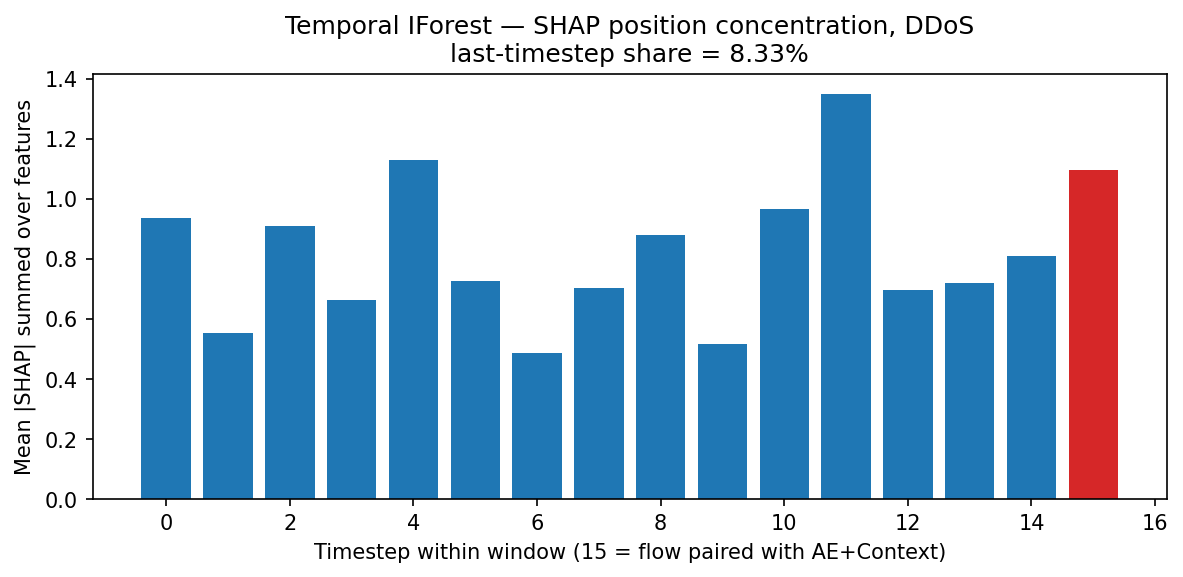
\includegraphics[width=0.48\textwidth,keepaspectratio]{../../data/explainability/cicids_temporal_shap/2/ddos_position_concentration.png}%
\hspace{0.02\textwidth}%
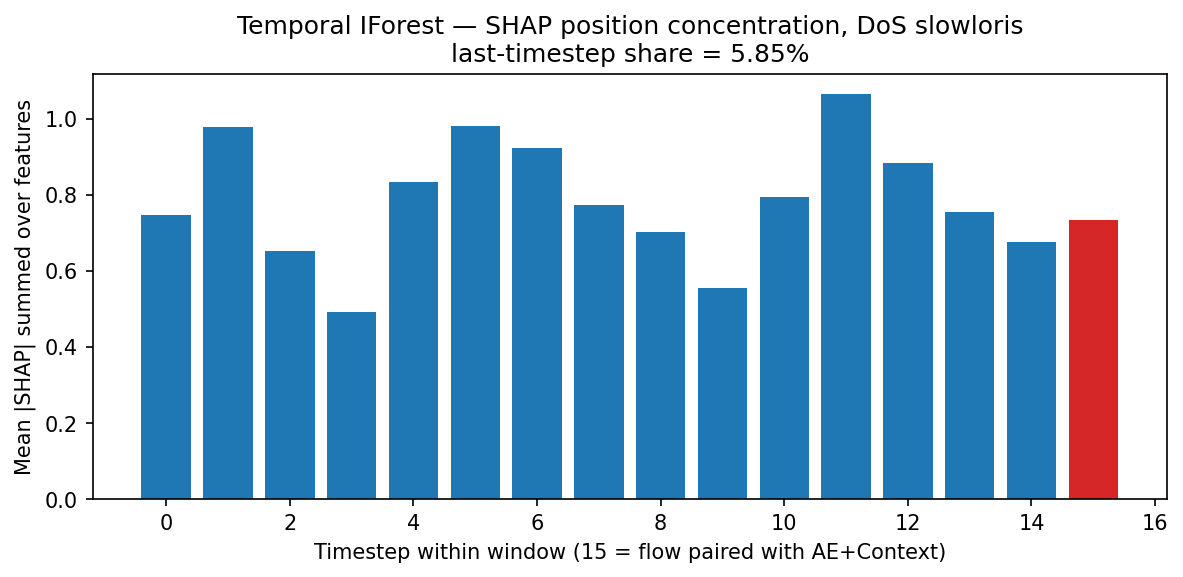
\includegraphics[width=0.48\textwidth,keepaspectratio]{../../data/explainability/cicids_temporal_shap/2/dos_slowloris_position_concentration.png}
\caption{Temporal IForest -- $|\text{SHAP}|$ mediu, sumat pe caracteristici, per pas temporal, ferestre DDoS (stânga) și ferestre DoS slowloris (dreapta). Ultimul pas temporal (bara roșie, 15) -- fluxul combinat cu scorul lui AE+Context în ansamblul propus -- nu poartă mai multă masă de atribuire decât orice altă poziție din fereastră, confirmând statistica sumară raportată în \S\ref{sec:explain-temporal-window}.}
\label{fig:explain-temporal-position-concentration}
\end{figure}

\begin{figure}[H]
\centering
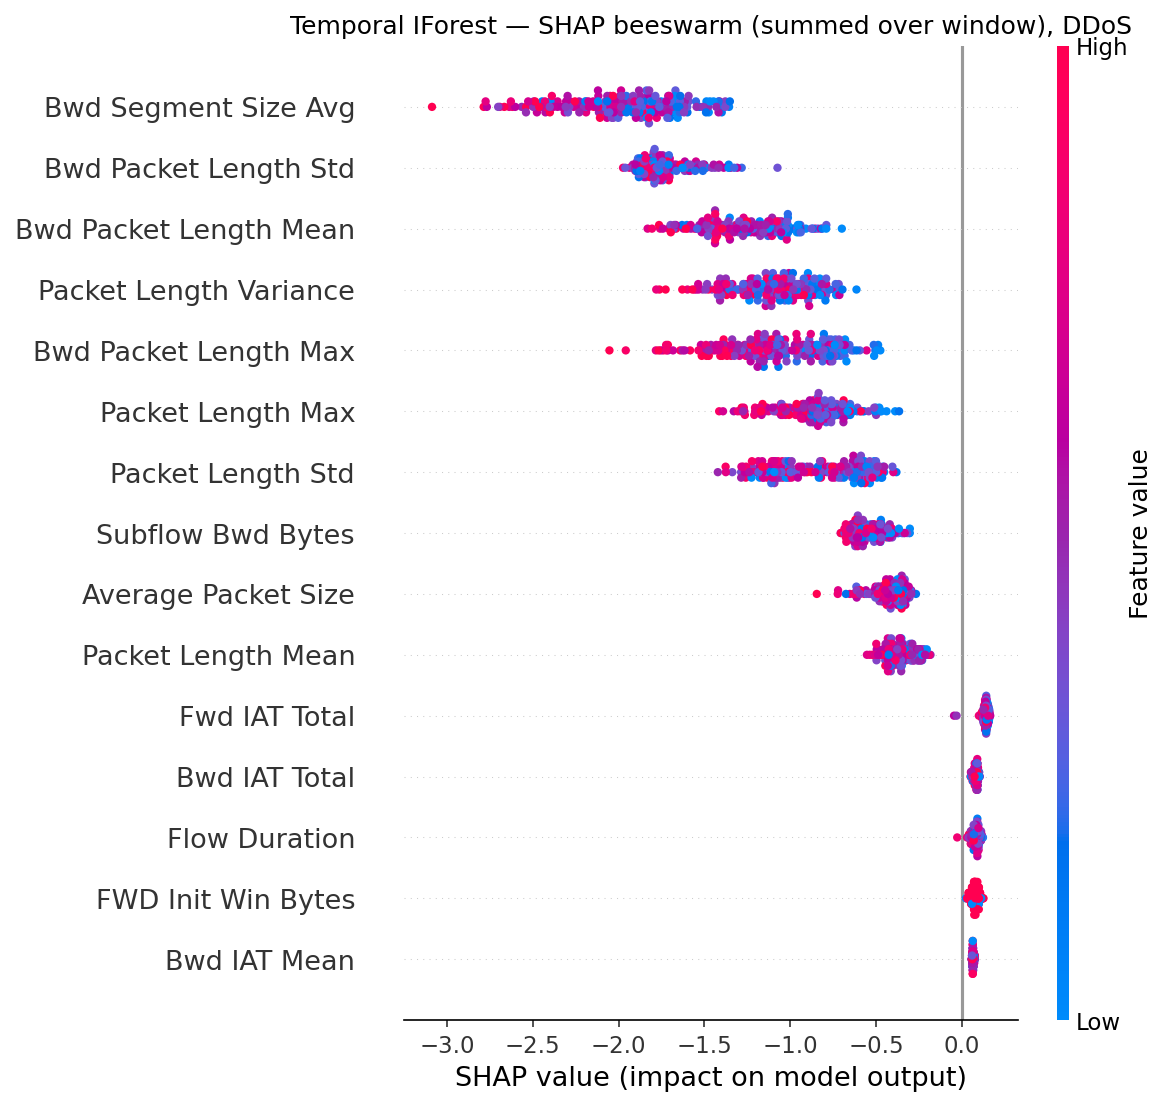
\includegraphics[width=0.48\textwidth,keepaspectratio]{../../data/explainability/cicids_temporal_shap/2/ddos_beeswarm.png}%
\hspace{0.02\textwidth}%
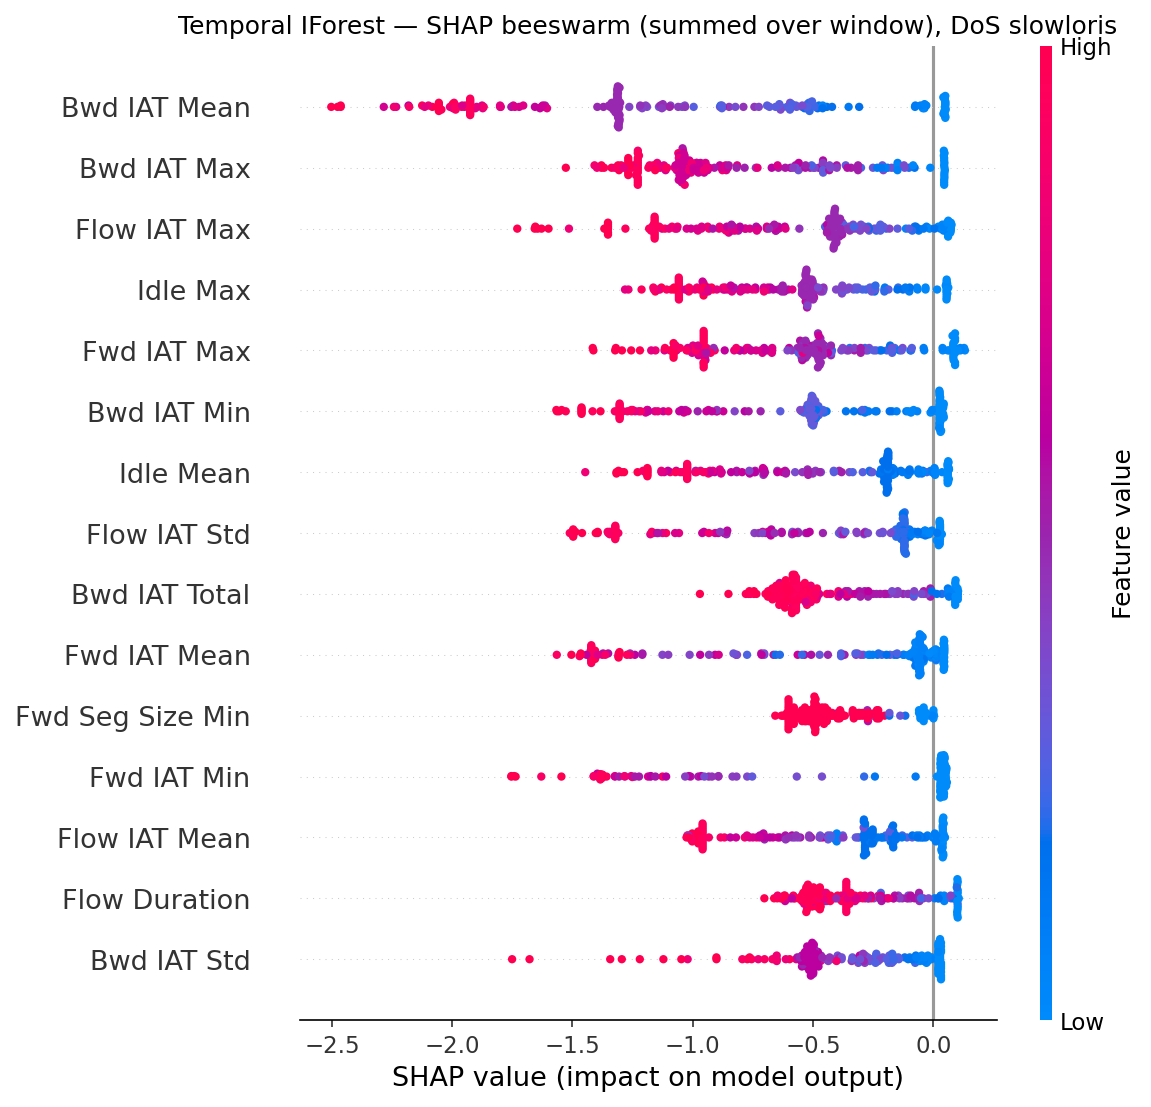
\includegraphics[width=0.48\textwidth,keepaspectratio]{../../data/explainability/cicids_temporal_shap/2/dos_slowloris_beeswarm.png}
\caption{Temporal IForest -- diagramă beeswarm SHAP per caracteristică, ferestre DDoS (stânga) și ferestre DoS slowloris (dreapta), colapsând axa celor 16 pași temporali prin sumarea contribuției SHAP a fiecărei caracteristici pe toată fereastra și colorând după valoarea medie a acelei caracteristici pe fereastră. DoS slowloris arată o relație monotonă clară -- valori mari ale timpului între sosiri (inter-arrival time) determină un SHAP puternic negativ (anormal), valorile mici împing spre zero -- consistent cu comportamentul lent, de menținere a conexiunii, după care este numit atacul. DDoS arată o relație valoare-semn mai zgomotoasă pentru caracteristicile sale de lungime a pachetelor pe direcția inversă, și o răspândire per fereastră mai largă decât sugerează, singură, imaginea de medii din Figura~\ref{fig:explain-temporal-shap}.}
\label{fig:explain-temporal-beeswarm}
\end{figure}

\chapter{Validarea Scorului Temporal IForest Sub Etichetare pe Ultimul Flux}
\label{ch:temporal-iforest-last-flow-validation}

Cifrele de AP per clasă arătate inițial folosesc o etichetă de fereastră "oricare-din-16", adică o fereastră este pozitivă dacă oricare din cele 16 fluxuri ale sale este un atac, etichetată cu tipul de atac majoritar.
Aceasta este mai permisivă decât etichetarea per flux față de care este evaluat AE+Context. Fiecare fereastră de test existentă a fost reetichetată în schimb cu eticheta reală proprie a fluxului \emph{ultim}, iar AP-ul per clasă a fost recalculat față de modelul deja antrenat, neschimbat, și scorurile sale existente.

\begin{center}
\begin{tabular}{@{}lccc@{}}
\toprule
 & AP (oricare-din-16) & AP (ultimul flux) & $n$ (ultimul flux) \\
\midrule
DDoS              & 0.9518 & 0.9515 & 95{,}123 \\
DoS GoldenEye     & 0.6278 & 0.6265 & 7{,}567 \\
DoS Slowhttptest  & 0.6851 & 0.6849 & 1{,}742 \\
DoS slowloris     & 0.6091 & 0.6077 & 4{,}001 \\
Heartbleed        & 0.5927 & 0.2892 & 11 \\
\bottomrule
\end{tabular}
\end{center}

Se observă că AP-ul rămâne practic neschimbat pentru toate cele patru clase țintă sub etichetarea mai strictă, confirmând că scorul este informativ despre statusul propriu al ultimului flux, nu un artefact al etichetării mai permisive.
Heartbleed scade brusc, dar pe doar 11 fluxuri reale -- întreaga sa populație de test -- deci este exclus din ansamblu și tratat ca provizoriu, consistent cu tratamentul său rezervat din Capitolul~\ref{ch:results}.

\chapter{Alinierea Scorurilor și Eșecul Standardizării \texorpdfstring{$z$}{z} pentru Ansamblul AE+Context + Temporal IForest}
\label{ch:ensemble-score-alignment}

Întrucât cele două pipeline-uri de preprocesare reordonează fluxurile diferit înainte de a-și salva propriile array-uri de test (AE+Context sortează global după marca temporală; Temporal IForest sortează per gazdă IP sursă), cele două array-uri de scoruri nu sunt aliniate index-cu-index și trebuie realiniate după identitatea fluxului, recuperând poziția originală a rândului fiecărui flux în intrarea comună, pre-sortare, a ambelor pipeline-uri.


Prima normalizare încercată, standardizarea $z$ (z-scoring) față de media și deviația standard proprii de antrenare benignă ale fiecărui model, s-a dovedit a fi o fundătură, nu un test autentic al niciunei reguli de combinare. Scorurile $z$ de eroare de reconstrucție ale lui AE+Context au cozi extrem de grele (maxim $z \approx 2366$ pe setul de test, cu percentila 99.9 a fluxurilor \emph{benigne} singure deja la $z \approx 227$), în timp ce scorurile $z$ ale lui Temporal IForest rămân strâns mărginite (maxim $z \approx 21$). Sub normalizarea $z$, o mână de valori extreme ale lui AE+Context domină orice combinație liniară sau maxim, indiferent de ponderea alocată lui Temporal IForest: atât regula maximului, cât și fiecare pondere de votare testată au reprodus aproape exact clasamentul propriu al lui AE+Context per clasă (de exemplu, AP-ul GoldenEye a rămas la $0.215$--$0.216$ pe toate cele cinci ponderi, față de $0.215$ al lui AE+Context singur), fără a arăta nicio influență din scorul de sine stătător mult mai puternic al lui Temporal IForest, $0.627$, pe acea clasă. Acesta este un artefact de normalizare, nu o dovadă că metoda combinării nu ajută -- nu testează de fapt ipoteza ansamblului.

Înlocuirea standardizării $z$ cu normalizarea pe rang -- mapând fiecare scor de test la percentila sa în distribuția scorurilor proprii de antrenare benignă ale acelui model, prin funcția de distribuție cumulativă empirică (CDF) -- elimină această problemă prin construcție: fiecare scor normalizat este mărginit la $[0,1]$ indiferent cât de extremă este valoarea brută, deci coada niciunui model nu poate domina coada celuilalt prin simpla magnitudine.